%package list
\documentclass{article}
\usepackage[top=3cm, bottom=3cm, outer=3cm, inner=3cm]{geometry}
\usepackage{multicol}
\usepackage{graphicx}
\usepackage{url}
%\usepackage{cite}
\usepackage{hyperref}
\usepackage{array}
%\usepackage{multicol}
\newcolumntype{x}[1]{>{\centering\arraybackslash\hspace{0pt}}p{#1}}
\usepackage{natbib}
\usepackage{pdfpages}
\usepackage{multirow}
\usepackage[normalem]{ulem}
\useunder{\uline}{\ul}{}
\usepackage{svg}
\usepackage{xcolor}
\usepackage{listings}
\lstdefinestyle{ascii-tree}{
    literate={├}{|}1 {─}{--}1 {└}{+}1 
  }
\lstset{basicstyle=\ttfamily,
  showstringspaces=false,
  commentstyle=\color{red},
  keywordstyle=\color{blue}
}
%\usepackage{booktabs}
\usepackage{caption}
\usepackage{subcaption}
\usepackage{float}
\usepackage{array}

\newcolumntype{M}[1]{>{\centering\arraybackslash}m{#1}}
\newcolumntype{N}{@{}m{0pt}@{}}


%%%%%%%%%%%%%%%%%%%%%%%%%%%%%%%%%%%%%%%%%%%%%%%%%%%%%%%%%%%%%%%%%%%%%%%%%%%%
%%%%%%%%%%%%%%%%%%%%%%%%%%%%%%%%%%%%%%%%%%%%%%%%%%%%%%%%%%%%%%%%%%%%%%%%%%%%
\newcommand{\itemEmail}{rvaldiviase@unsa.edu.pe}
\newcommand{\itemStudent}{Ryan Fabian Valdivia Segovia}
\newcommand{\itemCourse}{Fundamentos de la programación 2}
\newcommand{\itemCourseCode}{1701213}
\newcommand{\itemSemester}{II}
\newcommand{\itemUniversity}{Universidad Nacional de San Agustín de Arequipa}
\newcommand{\itemFaculty}{Facultad de Ingeniería de Producción y Servicios}
\newcommand{\itemDepartment}{Departamento Académico de Ingeniería de Sistemas e Informática}
\newcommand{\itemSchool}{Escuela Profesional de Ingeniería de Sistemas}
\newcommand{\itemAcademic}{2023 - B}
\newcommand{\itemInput}{Del 18 de Octubre 2023}
\newcommand{\itemOutput}{Al 23 de Octubre 2023}
\newcommand{\itemPracticeNumber}{07}
\newcommand{\itemTheme}{Combinando Arreglos Estándar y ArrayList}
%%%%%%%%%%%%%%%%%%%%%%%%%%%%%%%%%%%%%%%%%%%%%%%%%%%%%%%%%%%%%%%%%%%%%%%%%%%%
%%%%%%%%%%%%%%%%%%%%%%%%%%%%%%%%%%%%%%%%%%%%%%%%%%%%%%%%%%%%%%%%%%%%%%%%%%%%

\usepackage[english,spanish]{babel}
\usepackage[utf8]{inputenc}
\AtBeginDocument{\selectlanguage{spanish}}
\renewcommand{\figurename}{Figura}
\renewcommand{\refname}{Referencias}
\renewcommand{\tablename}{Tabla} %esto no funciona cuando se usa babel
\AtBeginDocument{%
	\renewcommand\tablename{Tabla}
}

\usepackage{fancyhdr}
\pagestyle{fancy}
\fancyhf{}
\setlength{\headheight}{30pt}
\renewcommand{\headrulewidth}{1pt}
\renewcommand{\footrulewidth}{1pt}
\fancyhead[L]{\raisebox{-0.2\height}{
\includegraphics[width=3cm]{img/logo_episunsa.png}}}
\fancyhead[C]{\fontsize{7}{7}\selectfont	\itemUniversity \\ \itemFaculty \\ \itemDepartment \\ \itemSchool \\ \textbf{\itemCourse}}
\fancyhead[R]{\raisebox{-0.2\height}{
\includegraphics[width=1.2cm]{img/logo_abet}}}
\fancyfoot[L]{Estudiante Ryan Valdivia}
\fancyfoot[C]{\itemCourse}
\fancyfoot[R]{Página \thepage}

% para el codigo fuente
\usepackage{listings}
\usepackage{color, colortbl}
\definecolor{dkgreen}{rgb}{0,0.6,0}
\definecolor{gray}{rgb}{0.5,0.5,0.5}
\definecolor{mauve}{rgb}{0.58,0,0.82}
\definecolor{codebackground}{rgb}{0.95, 0.95, 0.92}
\definecolor{tablebackground}{rgb}{0.8, 0, 0}

\lstset{frame=tb,
	language=bash,
	aboveskip=3mm,
	belowskip=3mm,
	showstringspaces=false,
	columns=flexible,
	basicstyle={\small\ttfamily},
	numbers=none,
	numberstyle=\tiny\color{gray},
	keywordstyle=\color{blue},
	commentstyle=\color{dkgreen},
	stringstyle=\color{mauve},
	breaklines=true,
	breakatwhitespace=true,
	tabsize=3,
	backgroundcolor= \color{codebackground},
}

\begin{document}
	
	\vspace*{10px}
	
	\begin{center}	
		\fontsize{17}{17} \textbf{ Informe de Laboratorio \itemPracticeNumber}
	\end{center}
	\centerline{\textbf{\Large Tema: \itemTheme}}
	%\vspace*{0.5cm}	

	\begin{flushright}
		\begin{tabular}{|M{2.5cm}|N|}
			\hline 
			\rowcolor{tablebackground}
			\color{white} \textbf{Nota}  \\
			\hline 
			     \\[30pt]
			\hline 			
		\end{tabular}
	\end{flushright}	

	\begin{table}[H]
		\begin{tabular}{|x{4.7cm}|x{4.8cm}|x{4.8cm}|}
			\hline 
			\rowcolor{tablebackground}
			\color{white} \textbf{Estudiante} & \color{white}\textbf{Escuela}  & \color{white}\textbf{Asignatura}   \\
			\hline 
			{\itemStudent \par \itemEmail} & \itemSchool & {\itemCourse \par Semestre: \itemSemester \par Código: \itemCourseCode}     \\
			\hline 			
		\end{tabular}
	\end{table}		
	
	\begin{table}[H]
		\begin{tabular}{|x{4.7cm}|x{4.8cm}|x{4.8cm}|}
			\hline 
			\rowcolor{tablebackground}
			\color{white}\textbf{Laboratorio} & \color{white}\textbf{Tema}  & \color{white}\textbf{Duración}   \\
			\hline 
			\itemPracticeNumber & \itemTheme & 04 horas   \\
			\hline 
		\end{tabular}
	\end{table}
	
	\begin{table}[H]
		\begin{tabular}{|x{4.7cm}|x{4.8cm}|x{4.8cm}|}
			\hline 
			\rowcolor{tablebackground}
			\color{white}\textbf{Semestre académico} & \color{white}\textbf{Fecha de inicio}  & \color{white}\textbf{Fecha de entrega}   \\
			\hline 
			\itemAcademic & \itemInput &  \itemOutput  \\
			\hline 
		\end{tabular}
	\end{table}
	
	\section{Tarea}
	\begin{itemize}
		\subsection{Videojuego}
			\item Cree un Proyecto llamado Laboratorio7
			\item Usted deberá crear las dos clases Soldado.java y VideoJuego4.java. Puede reutilizar lo
desarrollado en Laboratorios anteriores.
			\item Del Soldado nos importa el nombre, puntos de vida, fila y columna (posición en el tablero).
			\item El juego se desarrollará en el mismo tablero de los laboratorios anteriores. Para el tablero
utilizar la estructura de datos más adecuada.
			\item Tendrá 2 Ejércitos (utilizar la estructura de datos más adecuada). Inicializar el tablero con n
soldados aleatorios entre 1 y 10 para cada Ejército. Cada soldado tendrá un nombre
autogenerado: Soldado0X1, Soldado1X1, etc., un valor de puntos de vida autogenerado
aleatoriamente [1..5], la fila y columna también autogenerados aleatoriamente (no puede
haber 2 soldados en el mismo cuadrado). Se debe mostrar el tablero con todos los soldados
creados y sus puntos de vida. Además de los datos del Soldado con mayor vida de cada ejército, el
promedio de puntos de vida de todos los soldados creados por ejército, los datos de todos los
soldados por ejército en el orden que fueron creados y un ranking de poder de todos los
soldados creados por ejército (del que tiene más nivel de vida al que tiene menos) usando diferentes algoritmos de ordenamiento. Finalmente, que muestre qué ejército ganará la
batalla (indicar la métrica usada para decidir al ganador de la batalla). Hacer el programa
iterativo.
	\end{itemize}
		
	\section{Equipos, materiales y temas utilizados}
	\begin{itemize}
		\item Sistema Operativo Windows 11 Home Single Language 64 bits 22621.2283
		\item VIM 9.0.
		\item Visual Studio Code 64 bits 1.82.2
		\item OpenJDK 64-Bits 11.0.16.1
		\item Git 2.41.0.windows.1
		\item Cuenta en GitHub con el correo institucional. 
	\end{itemize}
	
	\section{URL de Repositorio Github}
	\begin{itemize}
		\item URL del Repositorio GitHub para clonar o recuperar.
		\item \url{https://github.com/RyanValdivia/fp2-23b.git}
		\item URL para el laboratorio 07 en el Repositorio GitHub.
		\item \url{https://github.com/RyanValdivia/fp2-23b/tree/main/fase02/lab07}
	\end{itemize}
	
	\section{Actividades}
	\subsection{Actividad 1}
	
	\begin{itemize}	
		\item En primer lugar, realicé un commit conteniendo el código de la clase Soldado.java, requerido para la clase principal
	\end{itemize}	
	\begin{lstlisting}[language=bash,caption={Obteniendo la clase Soldado}][H]
		$ git log lab07
		commit 9228a8c7c441745ab690009dee69fb3e8bdae06b
		Author: RYAN VALDIVIA <rvaldiviase@unsa.edu.pe>
		Date:   Sat Oct 21 12:25:58 2023 -0500
			Copiando la clase Soldado y reciclando algo de codigo de laboratorios anteriores
	\end{lstlisting}
	\begin{itemize}	
		\item Conteniendo el siguiente código en la clase Soldado
	\end{itemize}
	\begin{lstlisting}[language=java,caption={Clase Soldado}, numbers=left][H]
public class Soldado {
    private String nombre;
    private int vida;
    private int fila;
    private int columna;
    private String bandera;

    public void setNombre(String s) {
        this.nombre = s;
    }

    public void setVida(int n) {
        this.vida = n;
    }

    public void setFila(int n) {
        this.fila = n;
    }

    public void setColumna(int n) {
        this.columna = n;
    }

    public void setBandera(String s) {
        this.bandera = s;
    }

    public String getNombre() {
        return nombre;
    }

    public int getVida() {
        return vida;
    }

    public int getFila() {
        return fila;
    }

    public int getColumna() {
        return columna;
    }

    public String getBandera() {
        return bandera;
    }
}
	\end{lstlisting}
	\begin{itemize}
		\item Cabe aclarar, que añadí un atributo de 'bandera', será utilizado más tarde.
		\item Además de reutilizar el sistema para obtener las coordenadas de los soldados de laboratorios anteriores.
	\end{itemize}
	\begin{lstlisting}[language=java,caption={Código parcial}, numbers=left][H]
	public static void main(String[] args) {
        Scanner sc = new Scanner(System.in);
        Soldado[][] tablero = new Soldado[10][10];
        int ej1 = (int) (Math.random() * 10 + 1);
        int ej2 = (int) (Math.random() * 10 + 1);
        int[] filas1 = numerosRandom(ej1);
        int[] columnas1 = numerosRandom(ej1);
        int[] filas2;
        int[] columnas2;
        do {
                filas2 = numerosRandom(ej2);
                columnas2 = numerosRandom(ej2);
        } while (!diffCoordenadas(filas1, filas2, columnas1, columnas2));
    }
    public static int[] numerosRandom(int q) {
        int[] nums = new int[q];
        for (int i = 0; i < nums.length; i++) {
            nums[i] = nums.length;
        }
        for (int i = 0; i < q; i++) {
            int n;
            do {
                n = (int) (Math.random() * 10);
            } while (estaEnArreglo(nums, n, i));
            nums[i] = n;
        }
        return nums;
    }

    public static boolean estaEnArreglo(int[] arreglo, int num, int indice) {
        for (int i = 0; i < indice; i++) {
            if (arreglo[i] == num) {
                return true;
            }
        }
        return false;
    }

    public static boolean diffCoordenadas(int[] filas1, int[] filas2, int[] columnas1, int[] columnas2) {
        if (filas1.length > filas2.length) {
            for (int i = 0; i < filas2.length; i++) {
                if (filas1[i] == filas2[i] && columnas1[i] == columnas2[i]) {
                    return false;
                }
            }
        } else {
            for (int i = 0; i < filas1.length; i++) {
                if (filas1[i] == filas2[i] && columnas1[i] == columnas2[i]) {
                    return false;
                }
            }
        }
        return true;
    }
    
	\end{lstlisting}
	\begin{itemize}	
		\item Donde, ya que me daban a elegir la estructura de datos más adecuada para el tablero, utilicé un arreglo bidimensional porque se me hacía más sencillo al momento de inicializar e instanciar el tablero.
		\item Posteriormente, creé e inicialicé mis dos ejércitos, para esto, utilicé arreglos simples, para mayor conveniencia. Utilizando un método para crear un arreglo en base a las coordenadas ya creadas antes.
	\end{itemize}
	\begin{lstlisting}[language=java,caption={Creando ejércitos}, numbers=left][H]
		Soldado[] ejercito1 = crearArreglo(filas1, columnas1, 1);
		Soldado[] ejercito2 = crearArreglo(filas2, columnas2, 2);
		
		public static Soldado[] crearArreglo(int[] x, int[] y, int nro) {
        int len = x.length;
        Soldado[] army = new Soldado[len];
        for (int i = 0; i < len; i++) {
            int v = (int) (Math.random() * 5 + 1);
            army[i] = new Soldado();
            army[i].setNombre("Soldado" + i + "X" + nro);
            army[i].setVida(v);
            army[i].setFila(x[i]);
            army[i].setColumna(y[i]);
            if (nro == 1) {
                army[i].setBandera("##########");
            } else {
                army[i].setBandera("**********");
            }
        }
        return army;
    		}
	\end{lstlisting}
	\begin{itemize}	
		\item Entonces, este método recibe las filas y columnas (coordenadas) y empieza a inicializar los soldados de ambos ejércitos, además de darle una bandera a cada soldado (esto con el propósito de diferenciarlos al momento de imprimir el tablero).
		\item Además, añadí un método para 'desplegar' cada ejército en el tablero, en base a los arreglos con cada ejército.
	\end{itemize}
	\begin{lstlisting}[language=java,caption={Desplegando los ejércitos}, numbers=left][H]
		desplegarEjercito(tablero, ejercito1);
    		desplegarEjercito(tablero, ejercito2);
    		
    	public static void desplegarEjercito(Soldado[][] table, Soldado[] ej) {
        for (int i = 0; i < ej.length; i++) {
            table[ej[i].getFila()][ej[i].getColumna()] = ej[i];
        }
    }
	\end{lstlisting}	
	\begin{itemize}	
		\item Este método toma el arreglo de Soldados y asigna la referencia de cada uno de los Soldados al tablero, en base a los atributos de coordenadas de cada Soldado.
	\end{itemize}
	\begin{lstlisting}[language=java,caption={Inicializar la lista}, numbers=left][H]
	 public static void inicializarLista(ArrayList<ArrayList<Soldado>> army) {
        for (int i = 0; i < 10; i++) {
            army.add(new ArrayList<>());
        }
        for (int i = 0; i < 10; i++) {
            for (int j = 0; j < 10; j++) {
                army.get(i).add(new Soldado());
                army.get(i).get(j).setNombre("          ");
            }
        }

    }
	\end{lstlisting}
	\begin{itemize}	
		\item Ahora solo falta inicializar el tablero, ya que por defecto, inician todas las entradas en 'null'.
	\end{itemize}
	\begin{lstlisting}[language=java,caption={Inicializando tablero}, numbers=left][H]
	 	inicializarEjercito(tablero);
	 
	 public static void inicializarEjercito(Soldado[][] table) {
        for (int i = 0; i < table.length; i++) {
            for (int j = 0; j < table[i].length; j++) {
                table[i][j] = new Soldado();
                table[i][j].setNombre("          ");
                table[i][j].setBandera("          ");
            }
        }
    }
	\end{lstlisting}
	\begin{itemize}	
		\item Este método inicializa todas las entradas del arreglo bidimensional, y les asigna atributos de nombre y bandera vacíos, esto con el propósito de facilitar la tarea de imprimir el tablero.
		\item Entonces, este método se llama antes de desplegar los ejércitos.
		\item A continuación, solo quedaba mostrar el tablero de juego, para lo cual reutilicé código de los laboratorios anteriores, mejorándolo para que sea mucho más bonito y funcional, mostrando información completa de los soldados, como sus puntos de vida, nombre y una bandera única por ejércitos, para diferenciar unos de los otros.
	\end{itemize}
	\begin{lstlisting}[language=java,caption={Mostrar el tablero}, numbers=left][H]
	 public static void mostrarTablero(Soldado[][] tb) {
        String vacio = "          ";
        System.out.println(crearTecho());
        for (int i = 0; i < tb.length; i++) {
            System.out.println(separadorSup());
            for (int j = 0; j < tb[i].length; j++) {
                if (j == tb[i].length - 1) {
                    System.out.print("| " + tb[i][j].getBandera() + " |\n");
                } else {
                    System.out.print("| " + tb[i][j].getBandera() + " ");
                }
            }
            for (int j = 0; j < tb[i].length; j++) {
                if (j == tb[i].length - 1) {
                    System.out.print("| " + tb[i][j].getNombre() + " |\n");
                } else {
                    System.out.print("| " + tb[i][j].getNombre() + " ");
                }
            }
            for (int j = 0; j < tb[i].length; j++) {
                if (tb[i][j].getVida() != 0) {
                    if (j == tb[i].length - 1) {
                        System.out.print("|    " + tb[i][j].getVida() + " HP" + "    |\n");
                    } else {
                        System.out.print("|    " + tb[i][j].getVida() + " HP" + "    ");
                    }
                } else {
                    if (j == tb[i].length - 1) {
                        System.out.print("| " + vacio + " |\n");
                    } else {
                        System.out.print("| " + vacio + " ");
                    }
                }
            }
            System.out.println(separadorInf());
        }
        System.out.println();
    }

    public static String crearTecho() {
        String franky = "";
        for (int i = 0; i < 131; i++) {
            franky += "_";
        }
        return franky;
    }

    public static String separadorInf() {
        String franky = "";
        for (int i = 0; i < 131; i++) {
            if (i % 13 == 0) {
                System.out.print("|");
            } else {
                System.out.print("_");
            }
        }
        return franky;
    }

    public static String separadorSup() {
        String franky = "";
        for (int i = 0; i < 131; i++) {
            if (i % 13 == 0) {
                System.out.print("|");
            } else {
                System.out.print(" ");
            }
        }
        return franky;
    }
	\end{lstlisting}
	
	\begin{itemize}
		\item Es así que el código realiza varios recorridos por fila, imprimiendo primero la bandera del soldado (dependiendo de a qué ejército pertenece), su nombre y su nivel de vida (siendo HP, Health Points).
		\item Imprimiendo lo siguiente al momento de ejecutar el código:
	\end{itemize}
	
	\begin{figure}[H]
		\centering
	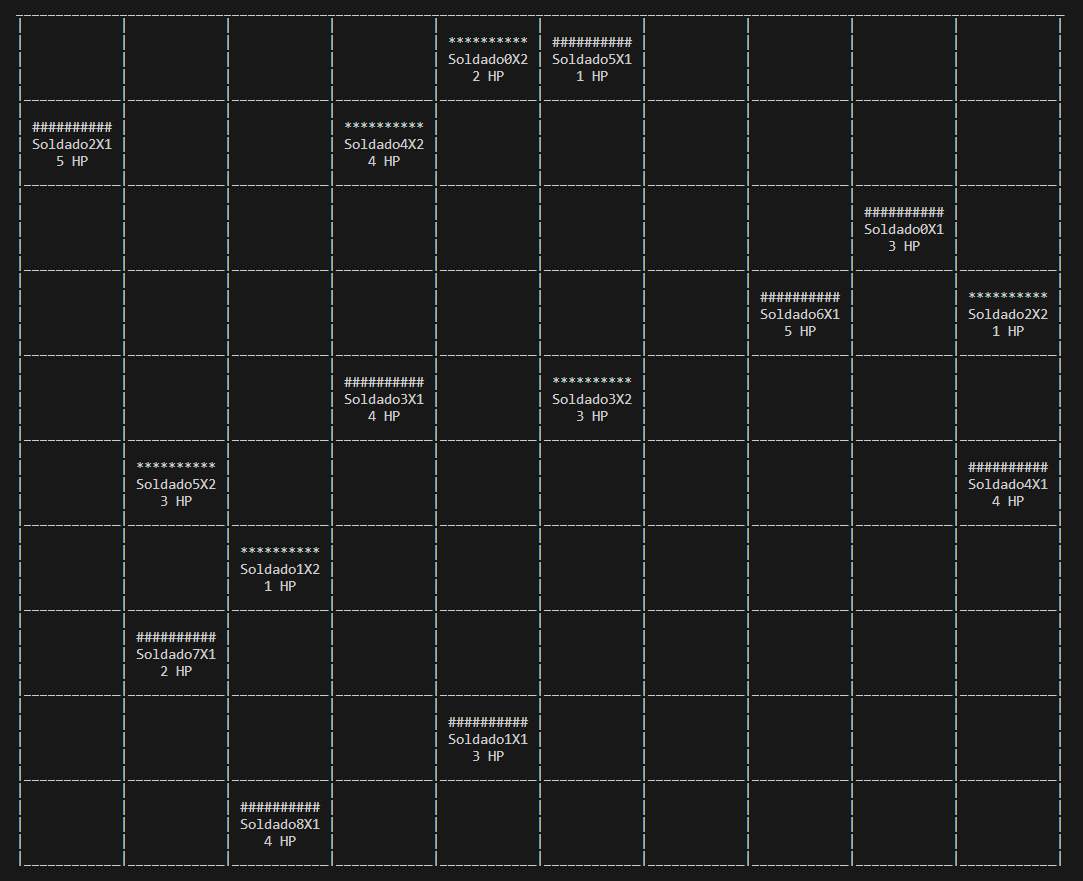
\includegraphics[width=0.8\textwidth,keepaspectratio]{img/captura1.png}
		%\includesvg{img/automata.svg}
		%\label{img:mot2}
		%\caption{Product backlog.}
	\end{figure}
	
	\begin{itemize}	
		\item Una vez terminado el tablero, pasé a trabajar el resto de requerimientos para el programa.
		\item Para mostrar el soldado con mayor vida del ejército, solo necesitaba recorrer el arreglo una vez para obtener el índice del objeto con mayor vida y mostrar sus datos, algo mucho más sencillo.
	\end{itemize}
	\begin{lstlisting}[language=java,caption={Soldado con mayor vida}, numbers=left][H]
	  public static void soldadoMayorVida(Soldado[] army, int ej) {
        int max = 0;
        for (int i = 0; i < army.length; i++) {
            if (army[i].getVida() > army[max].getVida()) {
                max = i;
            }
        }
        System.out.println("El soldado con mayor vida del ejercito " + ej + " es: ");
        mostrarSoldado(army, max);
        System.out.println();
     }
	\end{lstlisting}
	\begin{itemize}	
		\item Una vez encontrado el índice, solo debía mostrar el soldado de esa posición en el arreglo, para lo cuál, viendo que ese proceso sería algo que repita con frecuencia, decidí elaborar un método para mostrar un soldado.
	\end{itemize}
	\begin{lstlisting}[language=java,caption={Mostrar soldado}, numbers=left][H]
	  public static void mostrarSoldado(Soldado[] army, int i) {
        String columna;
        System.out.println("Nombre: " + army[i].getNombre());
        System.out.println("Vida: " + army[i].getVida() + " HP");
        switch (army[i].getColumna() + 1) {
            case 1:
                columna = "A";
                break;
            case 2:
                columna = "B";
                break;
            case 3:
                columna = "C";
                break;
            case 4:
                columna = "D";
                break;
            case 5:
                columna = "E";
                break;
            case 6:
                columna = "F";
                break;
            case 7:
                columna = "G";
                break;
            case 8:
                columna = "H";
                break;
            case 9:
                columna = "I";
                break;
            case 10:
                columna = "J";
                break;
            default:
                columna = "K";
                break;
        }
        System.out.println("Posicion: " + (army[i].getFila() + 1) + "-" + columna);
        System.out.println();
    }
    
	\end{lstlisting}
	
	
	\begin{itemize}	
		\item Después de ello, quedaba mostrar el total de vida de cada ejército y su vida promedio, para lo cual creé un método que imprimiera ambas cosas, recorriendo el arreglo una sola vez.
	\end{itemize}
	\begin{lstlisting}[language=java,caption={Vida total y promedio}, numbers=left][H]
	 public static void vidaPromedio(Soldado[] army, int ej) {
        int total = 0;
        for (Soldado s : army) {
            total += s.getVida();
        }
        System.out.println("La vida total del ejercito " + ej + " es: " + total);
        System.out.println("La vida promedio del ejercito " + ej + " es: " + total / (1.0 * army.length));
        System.out.println();
    }
	\end{lstlisting}
	\begin{itemize}
		\item Esto imprimía lo siguiente (Siguiendo con la ejecución de la captura anterior):
	\end{itemize}
	
	\begin{figure}[H]
		\centering
	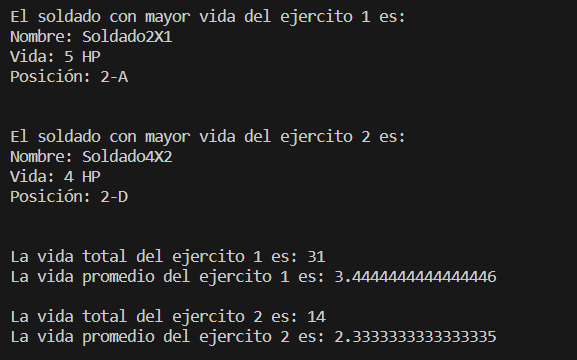
\includegraphics[width=0.8\textwidth,keepaspectratio]{img/captura2.png}
		%\includesvg{img/automata.svg}
		%\label{img:mot2}
		%\caption{Product backlog.}
	\end{figure}
	
	\begin{itemize}	
		\item Una vez terminado eso, seguía mostrar todos los soldados según el orden de creación, para eso, solo recorrí todo el arreglo y mostré cada soldado (para eso era el método anterior).
	\end{itemize}
	\begin{lstlisting}[language=java,caption={Mostrar ejército}, numbers=left][H]
	 public static void mostrarEjercito(Soldado[] army, int ej) {
        System.out.println("Ejercito " + ej);
        System.out.println(army[0].getBandera());
        for (int i = 0; i < army.length; i++) {
            mostrarSoldado(army, i);
        }
        System.out.println();
    }
	\end{lstlisting}
	\begin{itemize}
		\item Esto imprime lo siguiente:
	\end{itemize}
	\begin{figure}[H]
		\centering
	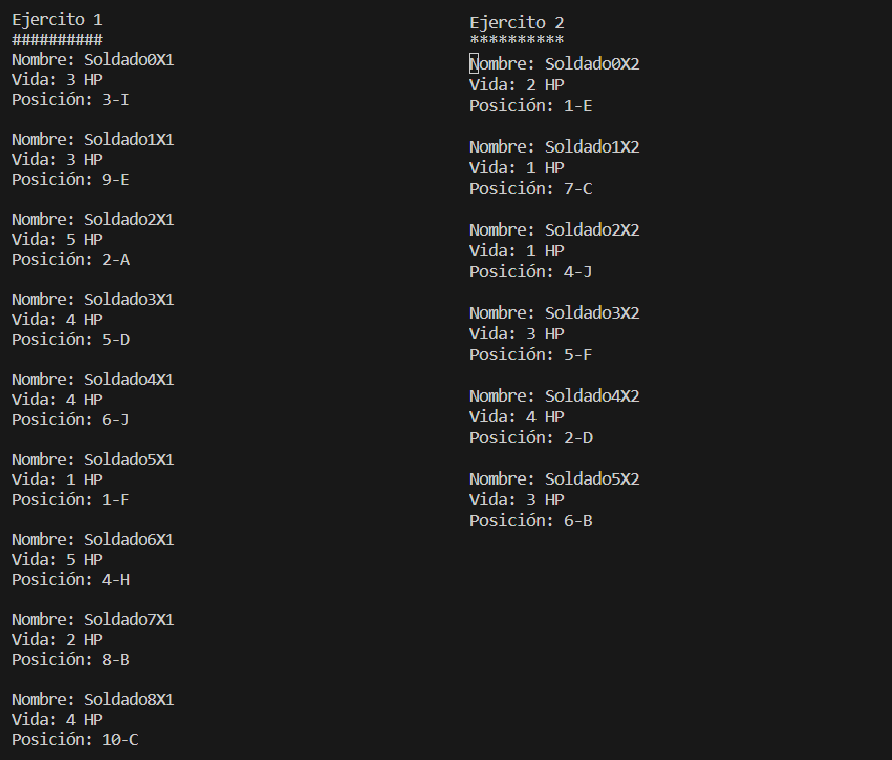
\includegraphics[width=0.8\textwidth,keepaspectratio]{img/captura3.png}
		%\includesvg{img/automata.svg}
		%\label{img:mot2}
		%\caption{Product backlog.}
	\end{figure}
	\begin{itemize}	
		\item Una vez terminado con esto, continué con realizar el ranking de Soldados según el nivel de vida (de mayor a menor), para esto, reciclé código de laboratorios anteriores para implementar los algoritmos de ordenamiento necesarios. Además de implementar un menú para escoger el algoritmo a usar.
	\end{itemize}
	
	\begin{lstlisting}[language=java,caption={Algoritmos de ordenamiento y ranking}, numbers=left][H]
	 System.out.println("Bajo que algoritmo de ordenamiento le gustaria ordenar su ejercito?");
     System.out.println("1. Ordenamiento por burbuja");
     System.out.println("2. Ordenamiento por insercion");
     switch (sc.nextInt()) {
     	case 1:
     		ordenamientoBurbuja(ejercito1);
       		ordenamientoBurbuja(ejercito2);
            break;
        case 2:
            ordenamientoInsercion(ejercito1);
            ordenamientoInsercion(ejercito2);
            break;
        default:
     }
     System.out.println();
            System.out.println("Ranking de ambos ejercitos del soldado con mayor a menor vida: \n");
            mostrarEjercito(ejercito1, 1);
            mostrarEjercito(ejercito2, 2);
    public static void ordenamientoInsercion(Soldado[] army) {
        for (int i = 1; i < army.length; i++) {
            Soldado valor = army[i];
            int j = i;
            for (j = i; 0 < j && army[j - 1].getVida() < valor.getVida(); j--) {
                army[j] = army[j - 1];
            }
            army[j] = valor;
        }
    }

    public static void ordenamientoBurbuja(Soldado[] army) {
        for (int i = 0; i < army.length; i++) {
            for (int j = 0; j < army.length - 1; j++) {
                if (army[j].getVida() < army[j + 1].getVida()) {
                    intercambiar(army, j, j + 1);
                }
            }
        }
    }

    public static void intercambiar(Soldado[] flota, int i, int j) {
        Soldado temp;
        temp = flota[i];
        flota[i] = flota[j];
        flota[j] = temp;
    }
	\end{lstlisting}
	\begin{itemize}	
		\item Entonces, se ordenan los ejércitos según el algoritmo seleccionado y posteriormente, se muestran en consola.
		\item Mostrando lo siguiente al momento de ejecutar.
	\end{itemize}
	
	\begin{figure}[H]
		\centering
	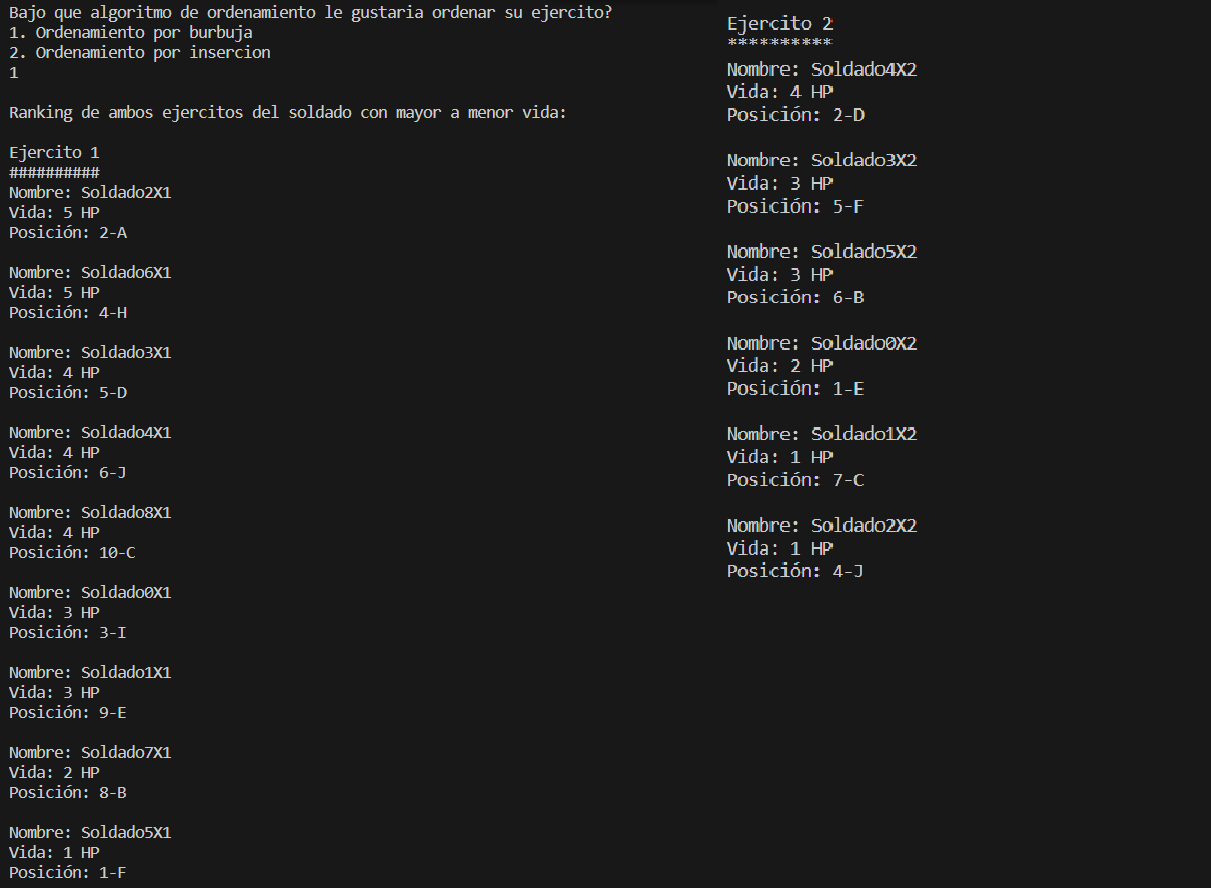
\includegraphics[width=0.8\textwidth,keepaspectratio]{img/captura4.png}
		%\includesvg{img/automata.svg}
		%\label{img:mot2}
		%\caption{Product backlog.}
	\end{figure}
	
	\begin{itemize}	
		\item A continuación falta lo último, que es determinar cuál de los dos ejércitos gana.
		\item Entonces, reciclé el mismo sistema de VideoJuegos anteriores, el ejército con mayor cantidad de vida gana.
	\end{itemize}
	
	\begin{lstlisting}[language=java,caption={Ejército ganador}, numbers=left][H]
	 public static void ejercitoGanador(Soldado[] f1, Soldado[] f2){
        int total1 = 0, total2 = 0;
        for(int i = 0; i < f1.length; i++){
            total1 += f1[i].getVida();
        }
        for(int i = 0; i < f2.length; i++){
            total2 += f2[i].getVida()
        }
        if(total1 > total2){
            System.out.println("El ejercito 1 es ganador!");
        }else if(total1 == total2){
            System.out.println("Hay empate!");
        }else{
            System.out.println("El ejercito 2 es ganador!");
        }
        System.out.println("Bajo la metrica de que ejercito tiene mas vida");
    }
	\end{lstlisting}
	\begin{itemize}	
		\item Finalmente, una vez todo está implementado, solo falta que el VideoJuego sea iterativo, para esto, puse todo el método main en un do-while, para que el usuario pueda volver a jugar si desea, o desea salir.
	\end{itemize}
	\begin{lstlisting}[language=java,caption={Método main final}, numbers=left][H]
	public static void main(String[] args) {
        Scanner sc = new Scanner(System.in);
        do {
            Soldado[][] tablero = new Soldado[10][10];
            int ej1 = (int) (Math.random() * 10 + 1);
            int ej2 = (int) (Math.random() * 10 + 1);
            int[] filas1 = numerosRandom(ej1);
            int[] columnas1 = numerosRandom(ej1);
            int[] filas2;
            int[] columnas2;
            do {
                filas2 = numerosRandom(ej2);
                columnas2 = numerosRandom(ej2);
            } while (!diffCoordenadas(filas1, filas2, columnas1, columnas2));
            Soldado[] ejercito1 = crearArreglo(filas1, columnas1, 1);
            Soldado[] ejercito2 = crearArreglo(filas2, columnas2, 2);
            inicializarEjercito(tablero);
            desplegarEjercito(tablero, ejercito1);
            desplegarEjercito(tablero, ejercito2);
            mostrarTablero(tablero);
            soldadoMayorVida(ejercito1, 1);
            soldadoMayorVida(ejercito2, 2);
            vidaPromedio(ejercito1, 1);
            vidaPromedio(ejercito2, 2);
            mostrarEjercito(ejercito1, 1);
            mostrarEjercito(ejercito2, 2);
            System.out.println("Bajo que algoritmo de ordenamiento le gustaria ordenar su ejercito?");
            System.out.println("1. Ordenamiento por burbuja");
            System.out.println("2. Ordenamiento por insercion");
            switch (sc.nextInt()) {
                case 1:
                    ordenamientoBurbuja(ejercito1);
                    ordenamientoBurbuja(ejercito2);
                    break;
                case 2:
                    ordenamientoInsercion(ejercito1);
                    ordenamientoInsercion(ejercito2);
                    break;
                default:
            }
            System.out.println();
            System.out.println("Ranking de ambos ejercitos del soldado con mayor a menor vida: \n");
            mostrarEjercito(ejercito1, 1);
            mostrarEjercito(ejercito2, 2);
            System.out.println("Presione q para salir, o cualquier otra tecla para volver a jugar");
        } while (!sc.next().equals("q"));

    }
	\end{lstlisting}
	\section{\textcolor{red}{Rúbricas}}
	
	\subsection{\textcolor{red}{Entregable Informe}}
	\begin{table}[H]
		\caption{Tipo de Informe}
		\setlength{\tabcolsep}{0.5em} % for the horizontal padding
		{\renewcommand{\arraystretch}{1.5}% for the vertical padding
		\begin{tabular}{|p{3cm}|p{12cm}|}
			\hline
			\multicolumn{2}{|c|}{\textbf{\textcolor{red}{Informe}}}  \\
			\hline 
			\textbf{\textcolor{red}{Latex}} & \textcolor{blue}{El informe está en formato PDF desde Latex,  con un formato limpio (buena presentación) y facil de leer.}   \\ 
			\hline 
			
			
		\end{tabular}
	}
	\end{table}
	
	\clearpage
	
	\subsection{\textcolor{red}{Rúbrica para el contenido del Informe y demostración}}
	\begin{itemize}			
		\item El alumno debe marcar o dejar en blanco en celdas de la columna \textbf{Checklist} si cumplio con el ítem correspondiente.
		\item Si un alumno supera la fecha de entrega,  su calificación será sobre la nota mínima aprobada, siempre y cuando cumpla con todos lo items.
		\item El alumno debe autocalificarse en la columna \textbf{Estudiante} de acuerdo a la siguiente tabla:
	
		\begin{table}[ht]
			\caption{Niveles de desempeño}
			\begin{center}
			\begin{tabular}{ccccc}
    			\hline
    			 & \multicolumn{4}{c}{Nivel}\\
    			\cline{1-5}
    			\textbf{Puntos} & Insatisfactorio 25\%& En Proceso 50\% & Satisfactorio 75\% & Sobresaliente 100\%\\
    			\textbf{2.0}&0.5&1.0&1.5&2.0\\
    			\textbf{4.0}&1.0&2.0&3.0&4.0\\
    		\hline
			\end{tabular}
		\end{center}
	\end{table}	
	
	\end{itemize}
	
	\begin{table}[H]
		\caption{Rúbrica para contenido del Informe y demostración}
		\setlength{\tabcolsep}{0.5em} % for the horizontal padding
		{\renewcommand{\arraystretch}{1.5}% for the vertical padding
		%\begin{center}
		\begin{tabular}{|p{2.7cm}|p{7cm}|x{1.3cm}|p{1.2cm}|p{1.5cm}|p{1.1cm}|}
			\hline
    		\multicolumn{2}{|c|}{Contenido y demostración} & Puntos & Checklist & Estudiante & Profesor\\
			\hline
			\textbf{1. GitHub} & Hay enlace URL activo del directorio para el  laboratorio hacia su repositorio GitHub con código fuente terminado y fácil de revisar. &2 &X &2 & \\ 
			\hline
			\textbf{2. Commits} &  Hay capturas de pantalla de los commits más importantes con sus explicaciones detalladas. (El profesor puede preguntar para refrendar calificación). &4 &X &2 & \\ 
			\hline 
			\textbf{3. Código fuente} &  Hay porciones de código fuente importantes con numeración y explicaciones detalladas de sus funciones. &2 &X &2 & \\ 
			\hline 
			\textbf{4. Ejecución} & Se incluyen ejecuciones/pruebas del código fuente  explicadas gradualmente. &2 &X &2 & \\ 
			\hline			
			\textbf{5. Pregunta} & Se responde con completitud a la pregunta formulada en la tarea.  (El profesor puede preguntar para refrendar calificación).  &2 &X &2 & \\ 
			\hline	
			\textbf{6. Fechas} & Las fechas de modificación del código fuente estan dentro de los plazos de fecha de entrega establecidos. &2 &X &2 & \\ 
			\hline 
			\textbf{7. Ortografía} & El documento no muestra errores ortográficos. &2 &X &2 & \\ 
			\hline 
			\textbf{8. Madurez} & El Informe muestra de manera general una evolución de la madurez del código fuente,  explicaciones puntuales pero precisas y un acabado impecable.   (El profesor puede preguntar para refrendar calificación).  &4 &X &4 & \\ 
			\hline
			\multicolumn{2}{|c|}{\textbf{Total}} &20 & &18 & \\ 
			\hline
		\end{tabular}
		%\end{center}
		%\label{tab:multicol}
		}
	\end{table}
	
\clearpage

\section{Referencias}
	\begin{itemize}
		\item Fundamentos de la programación 2 - Tópicos de la programación Orientada a Objetos (Marco Aedo)
	\end{itemize}
	
%\clearpage
%\bibliographystyle{apalike}
%\bibliographystyle{IEEEtranN}
%\bibliography{bibliography}
			
\end{document}
